%
%  $Description: Author guidelines and sample document in LaTeX 2.09$ 
%
%  $Author: ienne $
%  $Date: 1995/09/15 15:20:59 $
%  $Revision: 1.4 $
%

\documentclass[twoside,leqno,twocolumn]{article}  
\usepackage{siamdm} 
\usepackage{times}
\usepackage{amsmath}
\usepackage{amssymb}
\usepackage{graphicx}

\newcommand{\THOR}{{{\tt THOR}} }

\newcommand{\authornote}[1]{\footnote{Note to self: #1}}
\newcommand{\authorsnote}[1]{\authornote{#1}}
\newcommand{\com}[1]{{\small \textit{((#1))}}}

\newcommand{\union}{\cup}
\newcommand{\intersect}{\cap}
\newcommand{\Union}{\bigcup}
\newcommand{\Intersect}{\bigcap}
\newcommand{\bigvec}[1]{\mathop{\overrightarrow{#1}}}

\newcommand{\otimeshat}{\widehat{\otimes}}
\newcommand{\odothat}{\widehat{\odot}}

\newcommand{\prefsplit}[2]{#1 \succ #2}
\newcommand{\summary}{\hat{\sigma}}

\DeclareMathOperator*{\map}{map}
\DeclareMathOperator*{\worst}{worst}
\DeclareMathOperator*{\argmin}{argmin}
\DeclareMathOperator*{\argmax}{argmax}
\DeclareMathOperator{\TWOPT}{TWOPOINT}
\DeclareMathOperator{\cardinality}{cardinality}
\DeclareMathOperator{\hrect}{hrect}
\DeclareMathOperator{\child}{child}
\DeclareMathOperator{\visited}{visited}
\DeclareMathOperator{\unvisited}{unvisited}
\DeclareMathOperator{\prune}{prune}
\DeclareMathOperator{\IF}{if}
\DeclareMathOperator{\ATDISCRETION}{}

\newcommand{\fig}[1]{Figure~\ref{fig:#1}}

\newcommand{\Gnp}{\Psi}
\newcommand{\gnp}{\psi}

%\newcommand{\psty}{\scriptstyle}
\newcommand{\psty}{}
\newcommand{\X}{\\ \psty}
\newcommand{\x}{\X \hspace{0.13in}}
\newcommand{\xx}{\X \hspace{0.26in}}
\newcommand{\xxx}{\X \hspace{0.39in}}
\newcommand{\xxxx}{\X \hspace{0.52in}}

%\newcommand{\mysubsub}[1]{{\bf #1.}  }
%\newcommand{\mysub}[1]{{\bf #1.}  }
\newcommand{\mysubsub}[1]{\subsubsection{#1} }
\newcommand{\mysub}[1]{\subsection{#1} }

\newcommand{\defterm}[1]{{\bf #1}}
\newcommand{\nbody}{$N$-body}

\newcommand{\kdroot}[1]{#1^{\text{root}}}
\newcommand{\kdleft}[1]{#1^{\!L}}
\newcommand{\kdright}[1]{#1^{\!R}}
\newcommand{\kdparent}[1]{#1^{\!P}}

\newcommand{\lo}[1]{#1^{l}}
\newcommand{\up}[1]{#1^{u}}
\newcommand{\distlo}{\lo{d}}
\newcommand{\distup}{\up{d}}
\newcommand{\dist}[2]{d(#1,#2)}

%\newcommand{\myOp}[1]{\mathop{\bigotimes\nolimits\hspace{-0.045in}_{#1}}}
\newcommand{\nameOp}[2]{\mathop{#1\nolimits\!\!_{#2}}}
\newcommand{\nameop}[2]{{\scriptstyle\:}#1_{\!#2}}
\newcommand{\myOp}[1]{\nameOp{\bigotimes}{#1}}
%\newcommand{\myop}[1]{\otimes\hspace{-0.04in}_{#1}\hspace{0.03in}}
\newcommand{\myop}[1]{\nameop{\otimes}{#1}}
\newcommand{\myOutop}[1]{\nameOp{\bigodot}{#1}}
\newcommand{\myoutop}[1]{\nameop{\odot}{#1}}

\newcommand{\letterglob}{\psi}
\newcommand{\outglob}{\Psi}
\newcommand{\inglob}{\psi}
\newcommand{\Opglob}{\myOp{\letterglob}}
\newcommand{\opglob}{\myop{\letterglob}}
\newcommand{\fglob}{f_{\!\letterglob}}
\newcommand{\gglob}{g_{\!\letterglob}}
\newcommand{\canpruneglob}{C_{\!\letterglob}}
\newcommand{\deltaglob}{\summary_{\!\letterglob}}

\newcommand{\letterqr}{\rho}
\newcommand{\outqr}{\varrho}
\newcommand{\inqr}{\rho}
\newcommand{\Opqr}{\myOp{\letterqr}}
\newcommand{\opqr}{\myop{\letterqr}}
\newcommand{\fqr}{f_{\!\letterqr}}
\newcommand{\gqr}{g_{\!\letterqr}}

\newcommand{\letterqrv}{\vec{\rho}}
%\newcommand{\outqrv}{\vec{\rho}}
\newcommand{\inqrv}{\vec{\rho}}
%\newcommand{\fqrv}{f_{\letterqrv}}
%\newcommand{\gqrv}{g_{\letterqrv}}
\newcommand{\deltaqrv}{\summary_{\!\letterqrv}}
\newcommand{\canpruneqrv}{C_{\!\letterqrv}}
\newcommand{\identqr}{0_{\!\letterqrv}}
\newcommand{\varqrv}{\letterqrv^{\:C\!}}
\newcommand{\varqrvparent}{\letterqrv^{\:P\!}}

\newcommand{\lettermu}{\mu}
%\newcommand{\inmu}{\mu}
\newcommand{\inmu}{\mu}
\newcommand{\Outopmu}{\widehat{\nameOp{\bigodot}{\lettermu}}}%\mathop{\widehat{\bigodot\nolimits}\!\scriptstyle{\mu}}}
\newcommand{\outopmu}{\:\widehat{\odot}_{\!\mu}\:}
\newcommand{\Opmu}{\myOp{\lettermu}}
\newcommand{\opmu}{\myop{\lettermu}}
\newcommand{\fmu}{f_{\!\lettermu}}
\newcommand{\fmuv}{\vec{f_{\!\lettermu}}}
\newcommand{\deltamu}{\summary_{\!\lettermu}}
\newcommand{\canprunemu}{C_{\!\lettermu}}
\newcommand{\heurqr}{H}
\newcommand{\identmu}{0_{\lettermu}}
\newcommand{\varmuchild}{\lettermu^{\!C}}
\newcommand{\varmuparent}{\lettermu^{\!P}}

%\newcommand{\muparent}{\inmu_{\text{coarse}}}
%\newcommand{\muchild}{\inmu_{\text{children}}}
%\newcommand{\muvisit}{\inmu_{\text{visited}}}
%\newcommand{\muall}{\inmu_{\text{all}}}

%\newcommand{\hatpi}{\hat{\outpi}}
%\newcommand{\piparent}{\outpi_{\text{parent}}}

\newcommand{\letterstat}{s}
\newcommand{\namestat}[1]{\sigma_{\text{#1}}}
\newcommand{\outstat}{\sigma}
\newcommand{\instat}{s}
\newcommand{\Opstat}{\myOp{\letterstat}}
\newcommand{\opstat}{\myop{\letterstat}}
\newcommand{\fstat}{f_{\!\letterstat}}
\newcommand{\gstat}{g_{\!\letterstat}}

% Affinity propagation


\newcommand{\eqspace}{\!\!\!\!}
\newcommand{\true}{\text{true}}
\newcommand{\ocpos}[1]{c^{+}_{#1}}
\newcommand{\ocneg}[1]{c^{-}_{#1}}
\newcommand{\cpos}[2]{\ocpos{#1 \neq #2}}
\newcommand{\cneg}[2]{\ocneg{#1 \neq #2}}

\newcommand{\respo}[2]{R_{#1#2}}
\newcommand{\avail}[2]{A_{#1#2}}
\newcommand{\simil}[2]{S_{#1#2}}

\newcommand{\vecrho}{\vec{\rho}}
\newcommand{\vecalpha}{\vec{\alpha}}
\newcommand{\frho}[1]{\rho_{#1}}
\newcommand{\falpha}[1]{\alpha_{#1}}
\newcommand{\falphaj}[2]{\alpha_{#1[#2]}}

\newcommand{\falphamax}{\alpha^{u}}
\newcommand{\falphamin}{\alpha^{l}}
\newcommand{\frhomax}{\rho^{u}}
\newcommand{\frhomin}{\rho^{l}}

\newcommand{\alphacand}{v}


%\documentstyle[times,art10,twocolumn,latex8]{article}

%------------------------------------------------------------------------- 
% take the % away on next line to produce the final camera-ready version 
\pagestyle{empty}

%------------------------------------------------------------------------- 
\begin{document}

%\title{Framework for Fast Parallel Generalized N-Body Methods}
\title{Parallelization of Generalized $N$-Body Methods}

\author{Garrett F. Boyer, Ryan N. Riegel, Alexander G. Gray
\\ Georgia Institute of Technology
\\ Computational Science and Engineering
\\ 801 Atlantic Drive, Atlanta, GA
\\ garryb@cc.gatech.edu
\\
% For a paper whose authors are all at the same institution, 
% omit the following lines up until the closing ``}''.
% Additional authors and addresses can be added with ``\and'', 
% just like the second author.
\and
\\ Robert Nichol
\\ University of Portsmouth
\\ bob.nichol@port.ac.uk
}

\maketitle
\thispagestyle{empty}

\begin{abstract}
The multi-tree approach for accelerating data mining methods has spurred some of the fastest known solutions for a large class of fundamental methods previously considered impractical for massive datasets, including kernel density estimation, nearest-neighbor search, and spatial statistics.
We present a standard mathematical model that allows these problems to be scaled further via parallelization, without significant extra programmer effort.
With the framework, we derive a strategy for parallelization and describe our implementation, Tree High-Order Reduce or \THOR.
We demonstrate its applicability to severalrealistic sample data mining problems.
\end{abstract}

\section{Introduction}

Many problems in data mining nominally require an all-pairs analysis of metric data.
For a significant subclass of these problems, \defterm{generalized $N$-body problems} (GNP's), a higher-order divide and conquer technique can avoid nearly all computation by skipping combinations of regions with little mutual interaction.
Higher-order divide and conquer on metric\authorsnote{May need to explain what metric data is, depending on the type of reviewers to expect.} data typically utilizes metric trees, such as $kd$-trees \cite{preparata_kdtrees}, ball trees \cite{balltrees}, and cover trees \cite{covertrees}, to assist in dividing the data set into regions.
Such employment of trees is frequently called the \defterm{dual-tree} or the more generalized \defterm{multi-tree} approach.
This approach is used by some of the fastest known serial algorithms for many statistical and physical problems on metric data, such as bounded-error kernel density estimation \cite{gray_kde, lee_gauss1, lee_gauss2}, $n$-point correlation \cite{gray_nbody}, nearest neighbor search \cite{ryan_nips}, and more.

Nonetheless, as multi-core processors begin to dominate even commodity markets, even the fastest serial algorithms may not compete with a trivially parallelizable brute-force algorithm.
Additionally, and perhaps more importantly, some data sets are too massive to be practical on a single processor -- given enough processors, these problems may become practical.
Fortunately, multi-tree algorithms, owing to their divide-and-conquer nature, are in fact quite parallelizable.
We show that techniques that have long been used to parallelize the physical $N$-body force calculation methods can be, to an extent, applied to all GNP's.

Parallel programming is well-known for its significant cost in terms of development time, which is frequently far greater and more expensive than any achievable speedup.
However, we show that all second-order GNP's can be phrased as an instance of a generalized $N$-body algorithm, leading to an intriguing solution: Invest in a parallel solver for the general problem, requiring algorithm developers to provide only problem-specific portions.
In practice, this approach leads to efficient parallel and serial performance, and furthermore, the parallel algorithm in some cases takes less time to develop than a from-scratch serial algorithm.

%We describe in this paper both the formal problem generalization, and our implementation \THOR that executes dual-tree algorithms with two different expansion patterns.
%\authorsnote{Make sure it's clear at this point what is novel in my paper.  What should be clear is: (a) the mathematical model, and (b) its implementation in parallel.}

We present and justify three major claims.
We show a formal, unified model that solves all second-order generalized $N$-body problems, and respectively allows most dual-tree algorithms.
Second, we argue that programming in this unified model is not costly in developer time.
Finally, we show the inherent parallelism of our model by examining an implementation that uses well-known parallelization techniques.
\authorsnote{Cite some pivotal works on cache efficiency}
\authorsnote{Remind people that kd-trees are adaptive}
\authorsnote{Talk about our anti-undo policy}
\authorsnote{Try to appeal to people who don't really care about dual-tree algorithms, but just want raw parallelism.}

\section{Fast Dual-Tree Algorithms}

\begin{figure*}
  \begin{minipage}{6in}
    \begin{minipage}{2.5in}
      \begin{displaymath}
        \begin{array}[t]{l}
          \text{{\bf tpc} - Two-point correlation.}
          \X \text{function tpc}(X, Y)
          \x \text{if }\distup(\outstat(X), \outstat(Y)) > h\text{, return }0
          \x \text{if }\distlo(\outstat(X), \outstat(Y)) \leq h\text{, return } |X| \cdot |Y|
          \x \text{else if }|X| \geq |Y|\text{,}
          \xx \text{return tpc}(\kdleft{X}, Y, h) + \text{tpc}(\kdright{X}, Y, h)
          \x \text{else,}
          \xx \text{return tpc}(X, \kdleft{Y}, h) + \text{tpc}(X, \kdright{Y}, h)
        \end{array}
       \end{displaymath}
       \vspace{-.1in}
       \caption{\footnotesize \label{fig:allnntpc} Pseudocode for two simple dual-tree algorithms.
       $d$ signifies distance, and superscripts $l$ and $u$ refer, respectively, to lower and upper bounds.}
      \end{minipage}
      \begin{minipage}{3.0in}
       \begin{displaymath}
        \begin{array}[t]{l}
          \text{{\bf allnn} - Nearest-neighbor distances.}
          \X \text{for nodes }Q \subseteq \kdroot{Q}\text{, }a(Q) \gets \infty
          \X \text{procedure allnn}(Q,R)\text{,}
          \x \text{if }a(Q) < \distlo(\outstat(Q), \outstat(R))\text{, return}
          \x \text{else if }Q = \{q\} \text{ and } R = \{r\}\text{,}
          \xx a(\{q\}) \gets \min(a(\{q\}), \dist{q}{r})
          \x \text{else if }|Q| \geq |R|\text{,}
          \xx \text{allnn}(\kdleft{Q}, R); \text{ allnn}(\kdright{Q}, R)
          \xx a(Q) \gets \max(a(\kdleft{Q}), a(\kdright{Q}))
          \x \text{else, prioritize by node distance,}
          \xx \text{allnn}(Q, \kdleft{R}); \text{ allnn}(Q, \kdright{R})
        \end{array}
       \end{displaymath}
      \end{minipage}
  \end{minipage}
\end{figure*}

\mysub{Foundations}
\authornote{KD-tree figure goes here}
We briefly introduce the concept of metric trees and define some fundamental notation that we use throughout the paper.
Our notation considers tree node $X$ in a metric tree $\kdroot{X}$ to be a set of points.
These points lie in a metric space, such that a distance metric $\dist{x}{y}$ is commutative, satisfies the triangle inequality $\dist{x}{z} \leq \dist{x}{y} + \dist{y}{z}$, and is zero iff $x = y$.
For example, a $kd$-tree\cite{preparata_kdtrees}, as in \fig{kdtree}, is a binary tree that recursively divides the data along coordinate dimensions, and works with $L$ distance metrics such as Euclidean $L_2$.
Ball trees are binary and use bounding radii instead, and work with any metric space.
Cover trees are not binary and have a variable branching factor depending on the dimensionality of the data.
Quad-trees and oct-trees recursively bisect all coordinate dimensions for two- and three-dimensional vector spaces.
The choice of tree is often problem-specific, but generally results in a constant-factor rather than asymptotic complexity difference.
Our mathematical discussion, without loss of generality, treats non-binary trees as if they are binary for simplicity, with every internal node has partitioned $X = \kdleft{X} \union \kdright{X}$ and having parent $\kdparent{X} \supset X$.
Conceptually, a leaf is a single point $\{x\}$, though in practice multiple points may be grouped to amortize recursion overhead.

In all these trees, each node $X$ has summary information we label $\outstat(X)$.
Summary information includes the tree's bounding structure such as a hyper-rectangle or hyper-sphere, along with arbitrary summary statistics, such as mean, various moments, or other problem-specific information.
Bounds are a fundamental part of multi-tree algorithms, so we universally use superscripts $l$ and $u$ refer respectively to lower and upper bounds, which are often, as in the case of distance, obtained from the node's bounding structure.

\mysub{Single-tree versus dual-tree}
A common program structure, which we label \defterm{query-reference}, loops at the top level over a sequence of query points, and for each of those, considers all reference points with regard to the query.
An example, nearest neighbors, loops over many query points, and for each, loops over reference points to find the nearest one for that query.

A \defterm{single-tree} algorithm replaces the inner loop with a tree traversal, and skips parts of the tree that are irrelevant to the query, much like search in a binary search tree.
A \defterm{dual-tree} algorithm merges the two loops together and considers the entire computation a traversal over tree node pairs, forming a hierarchy over the Cartesian product of points.
The dual-tree algorithm \defterm{prunes} node pairs from consideration when possible, using summary information.
Although dual-tree algorithms can solve problems such as two-point correlation that have no actual differentiation between a query or reference point, the query-reference nomenclature simplifies our discourse with a minor loss in generality.
In many practical problems, the amount of computation that can be pruned is immense, reducing the complexity to $O(N log N)$, $O(N)$, or $O(N^{1+\epsilon})$ for $0 < \epsilon < 1$.
Although not tree-based algorithms, Strassen's\cite{strassen} matrix multiplication and Baeza-Yates\cite{baeza_yates} set-intersection algorithms also exhibit key features of higher-order divide and conquer.

For each query point, a single-tree algorithm must commence at the root of the tree and traverse towards the leaves or until pruning occurs, and is usually best $O(N log N)$.
A dual-tree algorithm instead considers the root-level nodes only with other root-level nodes, therefore amortizing the cost of considering the root-level nodes, and can be $O(N)$ in practice.
Empirical studies show that dual-tree algorithms significantly overtake similar single-tree algorithms for data sets larger than a threshold\authorsnote{I need to find the proximity project to justify this claim.}.
Such performance for large datasets make dual-tree algorithms a prime candidate for parallelization.

\mysub{Two-point correlation and range count}
The fundamental two-point-correlation statistic conceptually measures ``clumpiness'' and fractal dimension.
Its dual-tree algorithm is only a few lines of code and very simple to understand, yet is asymptotically fast in practice \cite{gray_nbody}.

Two-point correlation\footnote{A common formulation of two-point correlation skips redundant pairs, however, converting between the two is elementary algebra.} calculates the number of pairs of points within fixed radius $h$.
For data set $X$, radius $h$, and indicator function $I$, two-point correlation is
\[\sum_{x \in X} \sum_{y \in X} I(d(x, y) \leq h).\]
\noindent
The dual-tree algorithm in \fig{allnntpc} considers subset (node) pair $X$ and $Y$, returning immediately if all points are completely inside or outside the radius.
The asmyptotic speedup of this dual-tree algorithm, of the $O(N^{1+\epsilon})$ variety, was shown in \cite{gray_nbody}.

Two-point correlation is not necessarily a query-reference problem, since only a single result is required.
Its analog, range count, considers the number of points within the radius for each query,
\[\map_{q \in Q} \sum_{r \in R} I(d(q, r) \leq h).\]
Range count has a similar, but slightly more complex, dual-tree algorithm, that we enumerate in a later section.

\mysub{All nearest-neighbors}
In applications from manifold learning to classification, one computes the nearest point from reference set $R$ for each of a batch of queries $Q$.
We express this computation,
\[\map_{q \in Q} \argmin_{r \in R} d(q,r).\]
\noindent To achieve speedup, the dual-tree algorithm in \cite{ryan_nips} maintains for each query tree node $Q$ the furthest candidate neighbor distance, $a(Q)$.
If a set of references is farther away than this distance, no further exploration is required.

\mysub{Kernel density estimation}
By placing a kernel such as a multivariate Gaussian or Epanechnikov kernel at each data point, it is possible to estimate the overall probability density of a multi-dimensional data set.
Given a kernel $K$, data set $R$, and query points $Q$, calculate
\[\map_{q \in Q} \sum_{r \in R} K(q, r).\]
One of many dual-tree algorithms \cite{gray_kde, lee_gauss1, lee_gauss2} can be used to give a bounded relative-error approximations for each query point, by pruning subcomputations with acceptable error.

%\mysub{Affinity propagation}
%authorsnote: Affinity propagation has been removed, since the corresponding NIPS paper has been rejected and we have not the space to introduce a novel algorithm.

%Affinity propagation is a recent clustering technique that identifies exemplars in a data set, taking into account all point-to-point similarities\cite{affinity}.
%The similaritiy $\simil{i}{j}$ between points $x_i$ and $x_j$ is the negative squared distance or some other quantity to be maximized, with diagonals $\simil{i}{i}$ set to a parameter that controls the number of clusters.
%The algorithm maximizes the sum of similarities between each point and its chosen exemplar.
%If a metric space is defined over the points, one use the dual-tree algorithm in \cite{ryan_nips} to solve a modified version of the affinity propagation update steps,
%\[ \begin{array}{l}
%  \vecalpha \gets \map_{i} \argmin^2_{j} \!\left( \cpos{i}{j}(\cpos{i}{j}(\simil{i}{j} + \falphaj{i}{j}) - \frho{j}) - \simil{i}{j} \right)\! ,
%  \\
%  \vecrho \gets \map_{j} \sum_{i} \!\left( \cpos{i}{j}(\simil{i}{j} + \falphaj{i}{j}) \right)\!,
%\end{array} \]
%\noindent with $\ocpos{v}(x)$ being $\min(x, 0)$ for $v$ true and $x$ otherwise, and $\falphaj{i}{j}$ being the first minimum of $\falpha{i}$ when $i \neq j$ and the second otherwise.
%%These vectors are computed iteratively until convergence.
%%Exemplars are those points $j$ with $\frho{j}$ positive and each point belongs to the cluster defined by the exemplar closest to it.
%The algorithm uses $O(N)$ space and empirically took $O(N^{1.3})$ on three-dimensional points from a gravitational $N$-body particle simulation, compared to the existing $O(N^2)$ time and space method.

\mysub{Generalization}
All of the above problems have take the form of nested commutative, associative operators applied over an inner function.
Indeed, we later show this property is essential to both dual-tree algorithms and their parallelization.

\section{$N$-Body Particle Simulations}

$N$-body particle simulations comprise some of the best-studied parallel computing problems.
Most algorithms for efficient simulation use trees, and parallelization of these tree codes offers indispensible insight into that of generalized $N$-body problems.
The physical $N$-body problem models $N$ particles in an evolving system where each particle exerts force on all other particles.
Computational solutions break the simulation into discrete time steps, during which force is calculated as a query-reference generalized $N$-body problem,
\[\map_{q \in D} \sum_{r \in D} f(q,r),\]
\noindent where $f(q,r)$ is typically an inverse-squared-distance gravitational or Coulombic force.
Direct computation of the sum is $O(N^2)$ and has been one avenue of pursuit \cite{grape}.

However, the famous Barnes-Hut algorithm\cite{barnes_hut} and Fast Multipole Method\cite{greengard_fmm} achieve speedup by using trees to approximate distant interactions, and have been subject to enormous parallelization efforts.
Barnes-Hut\cite{barnes_hut} traverses an oct-tree\footnote{An oct-tree hierarchically divides all 3 dimensions at the midpoint.} to approximate force on each particle.
If query particle $q$ is further than parameter $\theta$ times the spatial width of the considered node, the force calculation is approximated by the node's center of mass.
Although Barnes-Hut is a single-tree algorithm, many aspects of its parallelization are applicable to the dual-tree case.

The Fast Multipole Method (FMM)\cite{greengard_fmm} achieves $O(N)$ on uniform distributions, but with a higher constant factor, by considering node-node interactions.
The FMM is indeed a special case of dual-tree algorithms due to its node-node computations.
However, its traversal pattern, often called a ``downwards pass,'' is quite specific and does not necessarily reflect the diversity of dual-tree problems.
Still, key parallelization insights are still applicable to dual-tree algorithms.

% \cite{singh95load} \cite{nyland93dataparallel} \cite{washington_nesl}

\section{Parallel Programming Productivity}

When approached with a potentially parallelizable problem, development time is typically far more expensive than CPU time.
Simplifying the process of developing parallel code has been a widespread goal of parallelization communities.

One approach is to create parallel programming languages or language extensions that allow a user to write serial or minimally parallel code and have it run on automatically on many processors.
These languages or extensions may provide terriffic performance for problems with regular access patterns, but leave the developer at the mercy of the language's abilities.
Generalized $N$-body problems rarely exhibit the type regularity of which these languages can take advantage.

However, NESL is a very high-level parallel programming language, semantically resembling ML, that is designed to handle irregular access pattern.
NESL sports parallel implementations of Barnes-Hut and the FMM \cite{blelloch_nbody}.
However, its explicit goal of rapid algorithm development for the benefit of teaching and experimentation overshadows the goal of fine-tuned production code.
We find direct implementation control to be advantageous for considering different communication or scheduling strategies, incorporating efficient machine-level code, and considering additional features like fault tolerance.
%Although it is fair to say that parallel programming languages have improved dramatically since then, there is still sparse literature on parallelizing $N$-body algorithms this way.

An increasingly popular approach involves generalizing a specific, yet diverse, class of problems.
One develops an arbitrarily fine-tuned implementation of the generalized problem in a fast language, but allow the user to plug in the algorithmic specifics.
Map-Reduce\cite{mapreduce} is a famous example for solving problems that process massive data sets through the three-step process of preprocessing, aggregating, and reduction.
By targetting only this class of problems, Map-Reduce can use optimally efficient data decomposition methods, out-of-core sorting algorithms, and mechanisms for fault-tolerance.
Additionally, very little work on the part of the programmer is needed, such that writing the parallel algorithm can be simpler than writing the serial algorithm.

Warren and Salmon\cite{warren95portable} made a similar argument over a decade ago when building a software framework for parallelizing oct-tree algorithms using a Hashed Oct-Tree method.
They created a fine-tuned implementation of single-tree algorithms based on previous Barnes-Hut work, but abstracted key points that can be replaced with custom code for different problems.
We do build on major points from both authors, prime figures in distributed-memory $N$-body algorithms.
However, dual-tree algorithms differ fundamentally from single-tree algorithms, and the Hashed Oct-Tree method is specific to oct-trees.

We show dual-tree algorithms have a novel generalization, of which we take advantage in order to create parallel code.
The developer needs only to focus on the interactions that occur among points and tree nodes, not on the details of the tree exploration or its parallelization.
We choose to implement \THOR in C++ owing to the availability of efficient compilers, low-level access to hardware, and efficient templating system.
Additionally, since programmers prefer to use common constructs such as vectors and lists over static bit-copiable structures, \THOR provides a scheme that takes advantage of C++ templates to implement serialization and deserialization of acyclic pointer graphs, using a templated object traversal.
Thus, we present \THOR as a ``quick and easy'' way to generate efficient parallel dual-tree algorithms.

\section{Dual-Tree Algorithm Framework}

Previously, we implied that a subclass of all-pairs computations are generalized $N$-body problems.
We begin to describe an extreme, though computationally unreasonable, generaliztion of $N$-body problems.
The class of \defterm{second-order reduce problems} is a type of all-pairs computation that is a superset of generalized $N$-body problems.
For commutative, associative operators $\bigotimes$ and $\bigodot$, postprocessing functions $h$ and $g$, inner function $f$, and data sets $X$ and $Y$, one computes,
\[\begin{array}{l}
  \displaystyle \Gnp(X, Y) = h(\gnp(X, Y)),
  \\
  \displaystyle \gnp(X, Y) = \bigodot_{x \in X} g\!\left(x, \bigotimes_{y \in Y} f(x, y) \right).
\end{array}\]
\noindent
For example, two-point correlation with radius $w$ is has,

\[\begin{array}{ccccl}
  %\mathcal{X} &\equiv& \mathcal{Y} &\equiv& \mathbb{R}^3
  %\\
  \bigodot &\equiv& \bigotimes &\equiv& \sum
  \\
  \multicolumn{3}{r}{f(x,y)} &\equiv& I(d(x,y) < w)
  \\
  \multicolumn{3}{r}{g(x, a)} &\equiv& a
  \\
  \multicolumn{3}{r}{h(a)} &\equiv& a
\end{array}\]

A second-order reduce problem is also a \defterm{generalized $N$-body problem} if for any partitioning $\kdleft{Y} \union \kdright{Y} = Y$,
\[\gnp(X,Y) = \gnp(X,\kdleft{Y}) \otimes \gnp(X,\kdright{Y}).\]
\noindent Note that similar decomposition of $X$ over $\bigodot$ is trivial by commutativity and associativity.
A simple generalized $N$-body problem, a \defterm{single-operator problem}, has $\bigodot = \bigotimes$ and a null $g$, such as two-point correlation above.

If $\bigodot$ is the higher-order operator $\map$ and $g$ is null, the above property is formally satisfied by rephrasing results as sets of key-value pairs, and the problem is a \defterm{query-reference GNP}.
For the sake of simplicity, we omit such formality, without loss of generality.

It is clear that {\em any} second-order reduce problem can be transformed into a query-reference GNP by replacing the outer operator with $\map$, and then treating both $g$ and $\odot$ as a postprocessing step.
Therefore, any framework that solves query-reference problems necessarily solves any second-order reduce problem.
Although \THOR's implementation does provide native support for both single-operator and query-reference problems, our discussion focuses on the more general query-reference problems.
We justify such omission since the transformation to the query-reference analog rarely results in an asymptotic difference in performance.
Nonetheless, we have shown that all generalized $N$-body problems can be expressed as query-reference problems, and proceed to show that the execution and pruning of most dual-tree algorithms can be generalized.

\mysub{The Generalized $N$-Body Algorithm}
Generalized $N$-body problems have a hierarchical computation,
\[
\gnp(X,Y) = \left\{ \begin{array}{lrr}
    f(x,y) & \multicolumn{2}{r}{\text{if }X = \{x\}\text{ and }Y = \{y\}\text{,}}
    \\
    \multicolumn{2}{l}{\gnp(\kdleft{X},Y) \otimes \gnp(\kdright{X}, Y)} & \text{if }\prefsplit{X}{Y}\text{,}
    \\
    \multicolumn{2}{l}{\gnp(X,\kdleft{Y}) \odot \gnp(X,\kdright{Y})} & \text{otherwise,}
  \end{array}
\right.
\]
\noindent
where $\prefsplit{X}{Y}$ specifies a recursion preference.
A single-tree algorithm is a special case where $\prefsplit{X}{Y} \equiv |X| > 1$, that is, $X$ is divided until individual queries are considered, after which $Y$ is recursed.
A dual-tree execution may use a heuristic such as $|X| \geq |Y|$ to prefer node pairs with approximately equal cardinality.
The generalized $N$-body algorithm initially considers the expression $\gnp(\kdroot{X}, \kdroot{Y})$, continually replacing any subexpression $\gnp(X, Y)$ with its aforementioned expansion.
The final expression forms an \defterm{expression tree} where leaves are of the form $f(x,y)$ and internal nodes are either $\odot$ or $\otimes$.

In the above, we only require that $X = \kdleft{X} \union \kdright{X}$ be a valid partitioning, not necessarily tree branches.
Trees are commonly used since they hierarchically group points that are likely to prune simultaneously as a group, i.e. a high correlation in pruning ability.

Dual-tree algorithms can use at-node statistics $\outstat(\cdot)$ to prove facts about node pairs at a higher level, and \defterm{prune} part of the expression tree.
A prune based only on statistics is an \defterm{intrinsic prune}.
In some cases, the results of computations outside of the currently considered pair can provide necessary evidence to prune.
For example, in all nearest-neighbors, a distant pair of nodes can be excluded if the query node's previously-calculated worst-case candidate neighbor is closer.
This prune is called an \defterm{extrinsic prune}.

%Sometimes the summary results of the entire problem imply that a subproblem needs no further consideration.
%Summary results can be aggregated bottom-up in the same manner the problem has been decomposed using some summary composition operator $A \otimeshat B \supseteq \{a \otimes b | a \in A, b \in B\}$ and likewise for $\odothat$.
%Unfortunately, these formal sets are infeasible to construct in practice, but can be bounded by considering single values that a represent a bound for a relevant part of the computation.
%An example is the upper bound nearest neighbor distance kept by nearest neighbors for each query node.
%For all-nearest-neighbors, this set is the set of all sets of possible key-value pairs representing query points and the corresponding possible nearest neighbor distances, each of which ranges continuously from 0 (the best distance possible) to the best candidate nearest neighbor distance.
%A prune is made by intersecting this with the similar set returned by $\summary(\outstat(X),\outstat(Y))$, and if the summary result set is unaffected, $(X,Y)$ may be skipped entirely.
%Unfortunately, it is infeasible to represent this construct directly in practice, so typically a single upper and/or lower bound is stored to summarize worst-case bounds.

%The generalized $N$-body algorithm begins with $\gnp(\kdroot{X},\kdroot{Y})$, and repeatedly replacing some $\gnp(X,Y)$ with one of its expansions.
%There is no one required exploration pattern.

It is worth noting that the generalized algorithm is agnostic to expansion pattern, that is, the order in which different subexpressions are replaced.
However, expansion pattern can have a significant, sometimes asymptotic, effect on run time.
With intrinsic pruning only, $\prefsplit{X}{Y}$ alone determines the asymptotic run time, so expansion pattern is irrelvant.
Extrinsically pruning problems that contentrate on spatially nearby computations may prefer a depth-first expansion along with a local ordering heuristic.
Others achieve good performance with a breadth-first expansion, which holistically refines the problem space.

Nearly all dual-tree algorithms we have encountered can be viewed as the algorithm above with intrinsic and extrinsic pruning.
However, the generalized algorithm does not explain the rich ``flow'' of data throughout an actual computation.
We next show, for query-reference problems, a set of generalized ``rules'' enumerating allowable ways in which results can be computed.

%Our paper treats parallel execution as an additional expansion pattern by noting that these subproblems can be considered independent and solved in parallel, given careful design choices.

%Ongoing research attempts to characterize all generalized N-body problems with rigorous mathematical formality; however, such rigorous formalization is outside the scope of this paper.
%Here, we postulate that all dual-tree algorithms fall into one or both of two categories: a single scalar or vector result summarizing all pairs of inputs, or an independent result for each query point computed against the entire reference set.

%A global reduction computes a single scalar or a vector of results that is constant with the number of data points.
%This type of problem is typically characterized by a single commutative, associative operator applied to pairs of inputs.
%Such problems include 2-point correlation, kernel-based data likelihood estimates, and the closest-pair problem.

%A query-reference problem alternatively computes a result for each point in a query set.
%For each point in the query set, execute a commutative, associative operator over every element in a reference set.
%These problems include such fundamental problems as all-nearest-neighbors, kernel density estimation, the testing phase of most nonparametric classification methods, matrix-vector multiplication, and many more.

%\subsection{Single-Operator Reduce Problems}
%
%A \defterm{single-operator reduce problem} computes a single scalar or relatively small vector of results, taking as input two data sets and applying an aggregate commutative and associative operator to all pairs,
%\begin{eqnarray*}
%\outglob(X, Y) &=& \gglob(\inglob(X, Y)),
%\\
%\inglob(X, Y) &=& \Opglob_{(x, y) \in X \times Y} \fglob(x, y).
%\label{eqn:defglob}
%\end{eqnarray*}
%
%\noindent where $\gglob$ is a post-processing function (usually identity), $\Opglob$ is a commutative and associative operator, and $\fglob$ is an inner function.
%We can express two-point correlation,
%\[\begin{array}{rcl}
%\TWOPT(X, r) &\equiv& \inglob_r(X, X),
%\\
%\opglob &\equiv& +
%\\
%\fglob(x, y) &\equiv& I(d(x, y) < h).
%\end{array}\]
%
%\noindent We decompose $\inglob$ with the identities,
%\begin{eqnarray*}
%\inglob(X, Y) &=& \inglob(\kdleft{X}, Y) \opglob \inglob(\kdright{X}, Y),
%\\
%\inglob(X, Y) &=& \inglob(X, \kdleft{Y}) \opglob \inglob(X, \kdright{Y}).
%\label{eqn:divideglob}
%\end{eqnarray*}
%
%\noindent and can be computed bottom-up $\instat(X) = \instat(\kdleft{X}) \opstat \instat(\kdright{X})$.
%Intrinsic prunes are applied with the following rule,
%\begin{equation*}
%\text{if } \canpruneglob(\outstat(X), \outstat(Y)) \text{, then } \inglob(X, Y) = \deltaglob(\outstat(X), \outstat(Y))
%\label{eqn:intrinsic}
%\end{equation*}
%\noindent where $\canpruneglob$ is a Boolean indicator that a prune is possible i.e. the initial summary set is singleton, and $\deltaglob$ is the summary set's only element.
%
%The rules shown so far allow some software system to execute single-operator reduce problems with intrinsic prunes given definitions for the relevant functions and operators.
%For instance, a $kd$-tree-based two-point correlation $\TWOPT(X, h)= \outglob(X,X)$ is defined:
%\begin{eqnarray*}
%\label{eqn:tpc_gglob}
%\gglob(\inglob) &\equiv& \inglob
%\\
%\label{eqn:tpc_opglob}
%\opglob &\equiv& +
%\\
%\label{eqn:tpc_fglob}
%\fglob(x,y) &\equiv& I(\dist{x}{y} < h)
%\\
%\label{eqn:tpc_canpruneglob}
%\canpruneglob(\sigma(X), \sigma(Y))
%&\equiv&
%\begin{array}{l}\distup(\outstat(X),\outstat(Y)) < h \\ \vee \distlo(\outstat(X),\outstat(Y)) \geq h\end{array}
%\\
%\label{eqn:tpc_deltaglob}
%\deltaglob(\outstat(X),\outstat(Y)) &\equiv& \left\{ \begin{array}{l} 0 \text{ if } \distup(\outstat(X),\outstat(Y)) < h \\ |X|\cdot|Y| \text{ if } \distlo(\outstat(X),\outstat(Y)) \geq h \end{array}\right.
%\\
%\label{eqn:tpc_fstat}
%\fstat(x) &\equiv& (x,x)
%\\
%\label{eqn:tpc_opstat}
%\opstat(x) &\equiv& \left( \bigvec{\min} , \bigvec{\max} \right)
%\end{eqnarray*}
%\noindent The first three summarize the problem itself, with the next two specifying the pruning condition.
%The last two specify the construction of a bounding box, although this is automatic with $kd$-trees.
%Given a parallel execution system, the above is all the programmer needs to specify to have a fully parallelized two-point correlation.
%

%The model shown so far is limited to very simple dual-tree algorithms.
%First, we later discuss additions to allow for efficient computation of query-reference problems such as all-nearest-neighbors and density estimation.
%Additionally, many algorithms, such as nearest-neighbor, classification problems, and approximate density estimates, require information about previous pairwise computation in order to determine whether pruning is possible.
%Nonetheless, this simple model leads to effective parallelization of problems such as two-point correlation\footnote{list more}.

\subsection{Query-reference instrinsic pruning}
A query-reference problem computes for each query $q$,
\begin{eqnarray}
\outqr(q, R) &=& \gqr(q, \inqr(q, R)),
\\
\inqr(q, R) &=& \Opqr_{r \in R} \fqr(q, r).
\label{eqn:qrdef}
\end{eqnarray}

\noindent where $R$ is initially $\kdroot{R}$.
In addition to the classic \nbody\ force calculation problem, this encompasses all nearest-neighbors, k-nearest-neighbors classification, nonparametric Bayes classification, kernel density estimation, affinity propagation, and more.
Although each query is independent, speedup is achievable by considering queries {\it en masse}; that is, the contribution of a set of references might be shown to have an exact value for an entire distant set of queries.
A \defterm{mass result} $\inqrv(Q, R)$ is defined if it is acceptable to treat
\[
\forall q \in Q,~~ \inqr(q, R) \gets \inqrv(Q, R)
\]
\noindent
within the context of the entire computation.
Otherwise, $\inqrv(Q,R)$ is undefined.
Expressed in tree notation,
\begin{equation}
\text{if prune occurs for } \kdparent{Q} \supset Q \text{, then } \inqrv(Q, R) = \inqrv(\kdparent{Q}, R).
\label{eqn:qrvparent}
\end{equation}

\noindent
Note that $\inqrv$ must be defined for singleton queries, and a single-tree algorithm conceptually treates $\inqrv$ in only this way.
It is important to note that although a dual-tree algorithm recursively descends the query tree, there is no explicit data dependency within the query tree, except the ability to incorporate mass results pruned from a parent.
Our mathematical model leaves to the implementation how the query set is divided.
Both types of algorithms, though, perform divide and conquer with the reference tree,
\begin{equation}
\inqrv(Q, R) = \inqrv(Q, \kdleft{R}) \opqr \inqrv(Q, \kdright{R}),
\label{eqn:qrvcompose}
\end{equation}
\noindent perhaps with an intrinsic prune,
\begin{equation}
\text{if } \canpruneqrv(\outstat(Q), \outstat(R)) \text{, then } \inqrv(Q, R) = \deltaqrv(\outstat(Q), \outstat(R)).
\label{eqn:qrvprune}
\end{equation}

\noindent
with statistics $\outstat(Q)$ and $\outstat(R)$, an intrinsic prune indicator function $\canpruneqrv$, and intrinsic prune value $\deltaqrv$.
Statistics are frequently built from commutative, associative operators, and may also be built bottom-up,
\begin{eqnarray}
\outstat(X) &=& \gstat(\instat(X)),
\\
\instat(X) &=& \Opstat_{x \in X} \fstat(x),
\label{eqn:defstat}
\end{eqnarray}

\noindent
Range count, the query-reference analog to two-point correlation, is fully defined,
\begin{eqnarray*}
\gqr(q, \inqr) &\equiv& \inqr
\\
\opqr &\equiv& +
\\
\fqr(q,r) &\equiv& I(\dist{q}{r} < h)
\\
\canpruneqrv(\outstat(Q), \outstat(R))
&\equiv&
\begin{array}{l}\distup(\outstat(Q),\outstat(R)) < h \\ \vee \distlo(\outstat(Q),\outstat(R)) \geq h\end{array}
\\
\deltaqrv(\outstat(Q),\outstat(R)) &\equiv& \left\{ \begin{array}{l} 0 \text{ if } \distup(\outstat(Q),\outstat(R)) < h \\ |R| \text{ if } \distlo(\outstat(Q),\outstat(R)) \geq h \end{array}\right.
\end{eqnarray*}

\noindent
The two-point correlation is then the sum of $\outqr$ for all queries.
Equations \ref{eqn:qrdef} through \ref{eqn:defstat} thus express the data flow of any query-reference problem that prunes only intrinsically using arbitrary commutative, associative statistics.

\subsection{Query-Reference Extrinsic Prunes}

Extrinsic pruning in a query-reference problems is a more complex process, but can still be represented in a general fashion.
We define \defterm{query summary results} $\inmu(Q, R)$ as a compact summary of previous computations relevant for the computation $(Q,R)$.
Checking for an extrinsic pruning desires the value of $\inmu(Q, \kdroot{R})$ to view the subcomputation in context of all reference nodes, not just the one considered.
After exhaustive computation, an \defterm{ideal} value may be computed,
\begin{equation*}
\inmu(Q, R) \gets \Outopmu_{q \in Q} \fmu(q, \inqr(q, R)).
\end{equation*}

\noindent for $\Outopmu$ a commutative and associative operator that merges representative summary results among queries.
For nearest neighbors, $\fmu(q, \inqr(q, R)) \equiv \inqr(q, R)$ and $\Outopmu \equiv \max$, in other words, the farthest candidate nearest neighbor.
%Although the generalized $N$-body algorithm states that summary results are built in the same structure as the refinement pattern, practical considerations encourage storing at each query node the best possible bounds for that node; for this reason, we start with this rather contrived definition.
We can merge subcomputations for disjoint query sets trivially,
\begin{equation}
\inmu(Q_1 \union Q_2, R) \gets \inmu(Q_1, R) \outopmu \inmu(Q_1, R).
\label{eqn:muchild}
\end{equation}

\noindent
The value of $\inmu(Q, \kdroot{R})$ is then used to make pruning decisions via the extrinsic prune check $\canprunemu(\outstat(Q), \outstat(R), \inmu(Q, \kdroot{R}))$.

During computation, the ideal value is not attainable since the final computation's value $\outqr(q, \kdroot{R})$ is obviously not known.
Before exploring a node pair, it is necessary to bound $\inmu$ from summary statistics,
\begin{equation}
\inmu(Q, R) \gets \deltamu(\outstat(Q), \outstat(R)).
\label{eqn:mudelta}
\end{equation}

\noindent
where $\deltamu$ is a pessimistic bound on pruning information.
For all nearest neighbors, this might be an upper-bound node-to-node distance, although the previous nearest-neighbors implementation treates unseen node pairs as being infinite distance apart.

Next, if we know $\inmu$ for disjoint reference sets, we may pessimistically compose them in a way analagous to the original $\Opqr$,
\begin{equation}
\inmu(Q, R_1 \union R_2) \gets \inmu(Q, R_1) \opmu \inmu(Q, R_1).
\label{eqn:mucompose}
\end{equation}

\noindent
It is important to note that the above composition may be quite pessimistic.
$\Outopmu$ takes the worst-case values from each query, and the above would compose those values even if the two values occured at different query points.
In practice, this pessimism is a necessary evil to avoid deeper traversal.
%For example, if $\inmu$ is an upper bound on a probability density contribution, summing the upper bounds neglects the possibility of having the upper bound appear at different query points for the two subcomputations.
%\authornote{Elaborate more, or make less comments.  Actually, this might want a proof.}

Next, an exact $\inqrv(Q, R)$ may be defined because this computation was pruned.
Ultimately $\inqrv(Q, R)$ will be propagated to individual queries, but until that happens, we bound the prune's worst-case contribution,
\begin{equation}
\inmu(Q, R) \gets \fmuv(\outstat(Q), \inqrv(Q, R)).
\label{eqn:muprune}
\end{equation}

\noindent
A simple matter, the summary information for any set of queries must necessary reflect all contained queries.
When no other information is available, we must resort to this rule, especially when performing depth-first expansions,
\begin{equation}
\inmu(Q, R) \gets \inmu(\kdparent{Q}, R) \text{ if } \kdparent{Q} \supset Q.
\label{eqn:muparent}
\end{equation}

\mysubsub{Quality}
A final note is that extrinsic pruning requires ``high-quality'' values of $\inmu$, that is, values that approach the aforementioned ideal value.
Although the quality of $\lettermu$ generally increases as more node pairs are explored, the order of exploration may help the value converge much faster.
The distribution of useful information over the space of node pairs is highly non-uniform in efficient dual-tree problems.
Prioritization is then used to concentrate on node pairs with higher potential information yield.
We introduce a heuristic function $\heurqr(\outstat(Q),\outstat(R))$ that returns a real value, such that lower values are explored first.

We believe that the above allows $\lettermu$ to be computed via the tree structure in any way that considers queries independent and involves commutative, associative operators.
For instance, finding all nearest neighbor distances then becomes,
\begin{eqnarray*}
\gqr(q, \inqr) &\equiv& \inqr
\\
\opqr &\equiv& \min
\\
\fqr(q,r) &\equiv& \dist{q}{r}
\\
\heurqr(\outstat(Q),\outstat(R)) &\equiv& \distlo(\outstat(Q), \outstat(R))
\\
\canprunemu(\outstat(Q), \outstat(R), \lettermu)
 &\equiv& \lettermu < \distlo(\outstat(Q), \outstat(R))
\\
\deltaqrv(\outstat(Q),\outstat(R)) &\equiv& \infty
\\
\outopmu &\equiv& \max
\\
\opmu &\equiv& \min
\\
\fmu(q, \letterqr) &\equiv& \letterqr
\\
\fmuv(\outstat(Q), \letterqrv) &\equiv& \letterqrv
\\
\deltamu(\outstat(Q),\outstat(R)) &\equiv& \distlo(\outstat(Q),\outstat(R))
\end{eqnarray*}

\noindent One small note is that in depth-first nearest-neighbor implementation, $\deltamu$ is typically ignored, i.e. treated as $\infty$, since it rarely provides useful information.
However, in breadth-first and other patterns, $\deltamu$ is essential.

\subsection{Execution}

To this point, we have defined many different ``rules'' that are assumed to be valid when computing a query-reference GNP.
\THOR must utilize an expansion strategy that applies these rules in order to solve a problem.

Previously, we showed locally-ordered depth-first implementations of two-point correlations and nearest neighbors in \fig{allnntpc}, that work by recursively dividing along the two trees.
\fig{dfe} shows the generalized depth-first dual-tree expansion algorithm that takes as input the data and functions of the generalized $N$-body problem.
This pseudocode, though heavily translated into C++, is present in \THOR to execute a locally-ordered depth-first expansion.

Some dual-tree algorithms achieve performance gains by maintaining a queue of node pairs to expand, rather than recursing immediately; however, this has worst-case $O(N^2)$ space.
\THOR implements a novel partially-recursive variant to reduce this to $O(N)$\footnote{
  In practice, pruning prevents the queues from approaching either of these worst-case sizes.}.
This expansion pattern mathematically differs from depth-first in the way summary results are computed.
Summary results are only accumulated from previous prunes and from the list of considered reference nodes.
Summary result quality is achieved by considering all references holistically at a finer and finer granularity.
On the other hand, depth-first expansion builds quality by visiting individual points first.
Although further discussion of the merits is warranted, it is beyond the scope of this paper\footnote{
  In short, the expansion strategy considers a query node with a list of reference nodes.
  While processing the list, creates similar lists for each of the query node's children.
  Each child is then explored recursively with its respective list.}.

\begin{figure}
\[
  \begin{array}[t]{l}
    \\ \text{Input:}\left(
        \begin{array}[c]{l}\kdroot{Q}, \kdroot{R}, \gqr, \opqr, \fqr, \deltaqrv, \\ \heurqr, \canpruneqrv, \canprunemu, \outopmu, \opmu, \fmuv, \deltamu\end{array}\right)
    \X \text{for all nodes } Q \in \kdroot{Q}\text{, } \varmuchild(Q) \gets \text{identity of }\Opmu
    \X \text{for all nodes } Q \in \kdroot{Q}\text{, } \varqrv(Q) \gets \text{identity of }\Opqr%\identqr
    \X \text{dfe}(\kdroot{Q}, \kdroot{R}, \text{identity of }\Opmu)
    \X \text{fixup}(\kdroot{Q}, \identqr)
    \X
    \X \text{procedure dfe}(Q, R, \varmuparent)\text{, \com{explore a node pair}}
    \x \text{\com{combine relevant $\lettermu$, Eqn~\ref{eqn:mucompose}}}
    %\x \!\!\!\begin{array}{lllll}
    %     \psty\inmu(Q,\kdroot{R}) &\psty\!\!\gets\!\!& \psty\varmuchild(Q) &\psty\!\!\opmu\!\!& \psty\fmuv(\outstat(Q), \varqrv(Q))
    %     \\              &\psty\!\!\opmu\!\!& \psty\varmuparent   &\psty\!\!\opmu\!\!& \psty\deltamu(\outstat(Q), \outstat(R))
    %   \end{array}
    \x \!\!\!\begin{array}{llll}
         \psty\lettermu &\psty\!\!\!\!\gets\!\!\!\!& \psty\varmuchild(Q)                     & \!\!\!\text{\com{bottom-up $\lettermu$, via Eqn~\ref{eqn:muchild}}}
         \\             &\psty\!\!\!\!\opmu\!\!\!\!& \psty\fmuv(\outstat(Q), \varqrv(Q))     & \!\!\!\text{\com{mass-result $\lettermu$, Eqn~\ref{eqn:muprune}}}
         \\             &\psty\!\!\!\!\opmu\!\!\!\!& \psty\deltamu(\outstat(Q), \outstat(R)) & \!\!\!\text{\com{node pair's $\lettermu$, Eqn~\ref{eqn:mudelta}}}
         \\             &\psty\!\!\!\!\opmu\!\!\!\!& \psty\varmuparent                       & \!\!\!\text{\com{unvisited $\lettermu$, Eqn~\ref{eqn:muparent}}}
       \end{array}
    \x \text{if } \exists q \exists r ~ Q = \{q\}\text{ and }R = \{r\}\text{,}
    \xx \text{\com{leaf-leaf interaction, Eqns \ref{eqn:qrdef}, \ref{eqn:qrvcompose}}}
    \xx \varqrv(\{q\}) \gets \varqrv(\{Q\}) \opqr \fqr(q, r)
    \x \text{else if } \canpruneqrv(\outstat(Q), \outstat(R))\text{ or }\canprunemu(\outstat(Q), \outstat(R), \lettermu)\text{,}
    \xx \text{\com{prune node-node interaction, Eqns \ref{eqn:qrvprune}, \ref{eqn:qrvcompose}}}
    \xx \varqrv(Q) \gets \varqrv(Q) \opqr \deltaqrv(\outstat(Q), \outstat(R))
    \x \text{else if } |Q| \geq |R|\text{,}
    \xx \text{\com{independently explore query children}}
    \xx \text{for } Q' \in \{\kdleft{Q}, \kdright{Q}\}\text{,}
    \xxx \text{\com{apply pruning information, Eqns \ref{eqn:qrvparent}, \ref{eqn:qrvcompose}}}
    \xxx \varqrv(Q') \gets \varqrv(Q') \opqr \varqrv(Q)
    \xxx \text{\com{recurse, by nature of dual-tree}}
    \xxx \text{dfe}(Q', R, \varmuparent)
    \xx \varqrv(Q) \gets \text{identity of }\Opqr
    \xx \text{\com{recompute high-quality $\lettermu$ bottom-up, Eqn~\ref{eqn:muchild}}}
    \xx \!\!\!\begin{array}{lll}
         \psty \varmuchild(Q) &\psty\!\!\gets\!\!&\psty (\varmuchild(\kdleft{Q})  \opmu \fmuv(\kdleft{Q}, \varqrv(\kdleft{Q})))
         \\          &\psty\!\!\outopmu\!\!&\psty (\varmuchild(\kdright{Q}) \opmu \fmuv(\kdright{Q}, \varqrv(\kdright{Q})))
        \end{array}
    \x \text{else}
    \xx \text{\com{explore reference children in heuristic order}}
    \xx (R_a, R_b) \gets \text{sort }(\kdleft{R}, \kdright{R})\text{ by }\lambda v ~ \heurqr(\outstat(Q), \outstat(v))
    \xx \text{\com{bound unvisited $\lettermu$ with statistics, Eqns \ref{eqn:mudelta}, \ref{eqn:mucompose}, \ref{eqn:muparent}}}
    \xx \text{dfe}(Q, R_a, \varmuparent \opmu \deltamu(\outstat(Q), \outstat(R_b))
    \xx \text{\com{use with parent's value of $\lettermu$, Eqn \ref{eqn:muparent}}}
    \xx \text{dfe}(Q, R_b, \varmuparent)
    \X
    \X \text{function fixup}(Q, \varqrvparent)\text{,}
    \x \text{\com{propagate mass results to leaves}}
    \x \varqrv(Q) \gets \varqrv(Q) \opqr \varqrvparent
    \x \text{if } \exists q ~ Q = \{q\}\text{,}
    \xx \outqr(q, \kdroot{R}) \gets \gqr(q, \varqrv(Q))
    \x \text{else,}
    \xx \text{fixup}(\kdleft{Q}, \varqrv(Q))
    \xx \text{fixup}(\kdright{Q}, \varqrv(Q))
  \end{array}
\]
\caption{\label{fig:dfe} The locally-ordered depth-first expansion algorithm for query-reference problems.
This subroutine is used internally in \THOR, though heavily translated to C++.
}
\end{figure}

So far, we have justified our first two claims about \THOR.
We have supported the completeness of our unified model with the existence of two generalized expansion patterns and two example algorithms, and will later show additional algorithms that have been ported.
Second, the ability to test new expansion patterns in a way that does not involve rewriting the code -- in fact, without any modifications at all -- shows that \THOR can actually be an aid in creating serial algorithms.
Next, we address the claim is that \THOR parallelizes these algorithms, and is just another execution style of the unified model.

\section{Parallel Execution}

Parallelization of {\em any} algorithm requires addressing how work is divided, what communication is necessary, and how work imbalances are kept to a minimum.
Decades of research into the parallelization of the Barnes-Hut and Fast Multipole algorithms gives insight into the parallelization of dual-tree algorithms.
However, we make significant deviations because of fundamental differences of dual-tree algorithms and the generality of both data structures and the problems solved.

\subsection{Task Decomposition}

A second-order generalized $N$-body problem, by definition, is decomposable in two orthogonal ways.
We may consider parallelization as an allowable expansion pattern permitted by the Generalized $N$-body Algorithm.
$\gnp(\kdroot{Q}, \kdroot{R})$ may be expanded into subproblems $(Q_1,R_1), (Q_2,R_2), ..., (Q_k, R_k)$ such that $\Union_{1 \leq i \leq k} (Q_i \times R_i) = \kdroot{Q} \times \kdroot{R}$.
Each subproblem can be executed in parallel, and merged using $\odot$ ($\map$ for query-reference problems) and $\otimes$.
Since the natural unit of subdivision for dual-tree algorithms is a tree node, we concentrate on decompositions where $Q_i$ and $R_i$ are tree nodes.

Although many decompositions are possible, we decompose the problem based only the query tree into tasks $(Q_1, \kdroot{R}), (Q_2, \kdroot{R}), ..., (Q_k, \kdroot{R})$.
Since $\odot$ is $\map$, all writable information is query-specific.
Thus, the query-based decomposition results in zero writes to shared data, and thus no write synchronization is necessary.
Furthermore, extrinsic pruning is highly dependent on the quality of query summary results for node $Q$, that is, $\inmu(Q, \kdroot{R})$.
Considering the entire reference tree on a single processor is advantageous because a high-quality value of $\lettermu$ can be computed on the local processor.

For single-operator problems like two-point correlation, one might consider decomposing both the query and reference tree because the only required communication is a single number.
Unfortunately, the execution time of distant node pairs tends to be orders of magnitude less that of nearby node pairs; such variance is extremely problematic for a generalized scheduler.
Our experience shows that a query-based decomposition scheme is typically quite manageable for even simple schedulers.
Finally, it is worth noting that past parallelization of both Barnes-Hut and the FMM universally divide queries among processors \cite{salmon_thesis, singh_thesis, liu94experiences}.

We define a task to be the solving of results for a subtree of queries.
These queries are processed using a standard serial solver, such as the aforementioned depth-first expansion in \fig{dfe}.
Typically, each processor executes several tasks over the course of the computation in order to allow dynamic task migration.

\subsection{Communication}

Communication is one of the fundamental factors inhibiting scalability of parallel algorithms, with experience showing it can be the primary scalability inhibitor for generalized $N$-body methods.
Although a query-based decomposition allows all writes to be independent, each task may need to consider interactions with arbitrary portions of the reference tree.
Consistent with previous literature\cite{salmon_thesis, singh_thesis}, we refer to this subset of reference nodes and points as a \defterm{locally essential tree}.
This is in contrast to the problem's \defterm{domain decomposition}, a one-to-one assignment of query tree nodes to processors.

\mysubsub{Domain decompositions}
A good domain decomposition for a single-tree algorithm promotes maximal overlap among the locally essential trees of query points, thereby minimizing the locally essential tree for that processor.
Salmon's earlier distributed implementations of Barnes-Hut \cite{salmon_thesis} decompose via orthogonal recursive bisection (ORB), or $kd$-tree that is balanced by estimated run time.
Each processor is assigned to a leaf in the orthogonal recursive bisection.
The spatial contiguity of the leaf hyper-rectangles generally leads to good overall spatial locality.

Singh et al. describe an alternate \defterm{cost-zones} decomposition\cite{singh95load} that instead sorts the query points along a sequential ordering of the oct-tree.
The points are then divided into contiguous segments with roughly equal estimated run time.
Singh et al. shows\cite{singh95load} that this technique typically performs better than the ORB decomposition since its decomposition is based off the same data structure of the data.

Not surprisingly, locality issues in dual-tree algorithms are very similar to those of dual-tree algorithms.
THOR combines the strengths from both ideas by simply balancing the $kd$-trees in a way that each processor can be assigned a tree node.
A lurking point is that if the query and reference data sets are not the same, it may be helpful to distribute both data sets using the same spatial divisions.
Our initial version builds each tree independently, but in the common case that there are significantly more queries than references, the extra communication overhead is quite small.
In a later section, we discuss dynamic adaptations that THOR performs when information about the relative amount of work is unavailable.

\mysubsub{Nature of communication}

In \THOR, interprocessor communication has two flavors.
First, within a single machine, multiple cores and processors are sharing local memory but may have local caches.
Modern multicore machines such as Intel's Core brand processors share L2 caches between consecutive nodes, and to maximize cache usage, it is best to assign these pairs similar chunks of the tree.
However, in small-scale SMP systems, we find dual-tree algorithms within a single query task have enough locality to ensure high cache hit rates, and thus low enough need for memory bandwidth, that little care is needed to reduce memory contention.

Singh in \cite{singh_thesis} argues that the high data requirements of $N$-body methods prevent efficient distributed-memory implementations, instead recommending costly shared-memory architectures to achieve parallelization.
However, several authors \cite{salmon_thesis, liu94experiences, salmon97parallel} have made successful implementations of the classic force-calculation methods.
Furthermore, generalized $N$-body problems have widely different computational characteristics.
In general, the most time consuming algorithms have relatively lower communication requirements relative to computation.
A low-dimensional nearest neighbor computation for 16 million three-dimensional points can be computed in under a minute on a single processor -- a single point-to-point transfer these points may take several times as long.
For the same data set, a two point correlation with a wide bandwidth may take hours, parallelizing extremely well.
Moreover, a nearest-neighbor computation for high-dimensional manifolds may also take hours and similarly parallelize well.
Nonetheless, several authors have made successful cluster implementations of both Barnes-Hut and the Fast Multipole Method.

Initially, Salmon\cite{salmon_thesis}, and Liu and Bhatt\cite{liu94experiences} promote the idea of sender-initiated communication.
In other words, each machine computes which of its own points and nodes belong to the locally essential trees of other machines, and sends them before computation begins.
By predicting needed data, no latency costs due to requesting remote data are paid, and therefore transfer time is the only limitation.
Such computation is possible since Barnes-Hut's pruning criterion is based only on the bounding box and distances of the cells.

Dual-tree algorithms may have diverse pruning criteria that cannot be predicted without actually beginning computation -- one example is a bounded-error kernel density estimation\cite{gray_kde}.
Salmon later describes\cite{salmon97parallel} a successful Barnes-Hut implementation that fetches data on demand, but avoids latency by grouping points into \defterm{blocks} of a fixed size.
In this context, the authors block data to allow an out-of-core $N$-body simulator, but also show it yields excellent parallel performance.
Such a blocking strategy is also the underlying mechanism behind shared-memory systems.
For these reasons, THOR utilizes an on-demand block-transfer strategy.
\authorsnote{I might briefly mention SAM, NESL, and eager consistency here, that are all related to this topic.}

\mysubsub{Distributed cache system}
Although entirely hidden from user code, \THOR's fundamental abstraction of shared data is the cached array.
A cached array is an array distributed in fixed-sized blocks, whose architecture is depicted in \fig{cache}.
One array contains points, with blocks 8 kilobytes or 100 points; a nodes array block has 2 kilobytes or 10 nodes\footnote{Block sizes in bytes depend on the communications network, on the order of latency times transfer rate.  The size of a point or varies based on dimensionality and extra statistics.}.
We separate nodes from points to allow independent block-size control and simpler programmability.
An element is accessed by explicitly locking and unlocking its block into memory.

\begin{figure}
  \hspace{-.17in}
  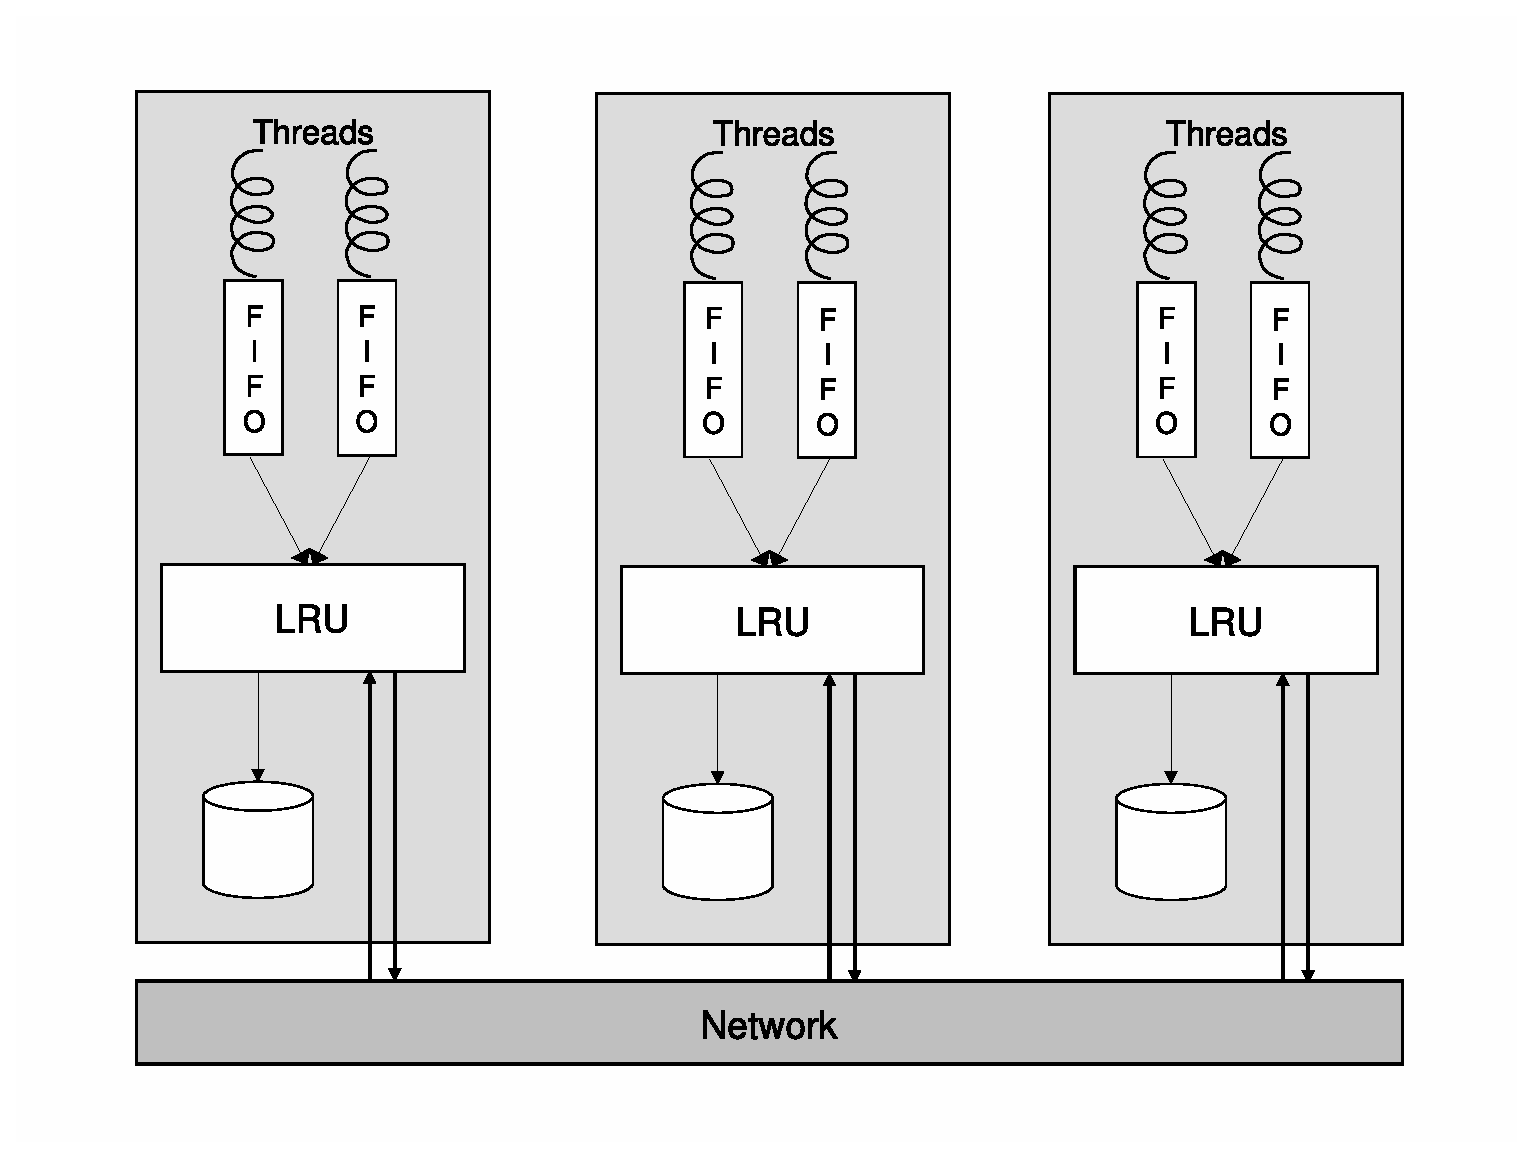
\includegraphics[width=3.5in,height=2.3in]{DistributedArchitecture.eps}
  \vspace{-.3in}
  \
  \caption{\label{fig:cache} A single distributed cache in THOR.}
\end{figure}

The main cache is a set-associative LRU cache\footnote{We use 16-block sets, although we omit for brevity empirical evidence suggesting diminished returns beyond 4 blocks.} that is shared among all threads.
For each block, the cache maintains the remote owner and whether it is in memory.
When a block is first accessed, a block is requested from its owner, and when unlocked, placed in the set-associative cache.
Infrequently used remote pages can be evicted from cache.

THOR uses a remarkably simple coherency protocol.
Simultaneous reads and writes to the same block are permitted if they are restricted to explicitly declared disjoint contiguous regions.
When the block is evicted, only these regions are written.
Consistency is ensured only at global synchronization points, occurring only before and after the GNP executes.

To avoid lock contention and caching overhead, each thread has a small (about 64 blocks) FIFO cache of blocks locked into the main cache.
THOR's dual-tree expansion code locks blocks into the FIFO cache\footnote{The FIFO cache's size places a hard limit on the number of active blocks.  64 blocks is quite generous for tree traversals.}.
Blocks are evicted to the set-associative cache in a round-robin fashion, skipping locked blocks.

\mysubsub{Data layout}
\THOR stores points are in tree-based skewed Morton ordering.
Additionally, we build the $kd$-tree such splits are aligned to block boundaries until a single block is reached, ensuring a one-to-one mapping between tree nodes and blocks of points.
Thus, storage spatial locality mirrors the metric spatial locality.
Tree nodes are stored pre-order, ensuring that subtrees correspond to contiguous ranges of nodes, and thus can be manipulated using our coherence model.

Nodes and points are then distributed block-by-block via the above domain decomposition.
If tree sections cross block boundaries, a tiebreaker is used.

\subsection{Scheduling}

\authorsnote{The scheduling subsection is weak at the moment and needs revising.}
Previous work \cite{salmon_thesis, singh_thesis} on scheduling $N$-body force calculation problems assume that relative run-time can be predicted from prior iterations.
Since \THOR aims to solve many problems that do not involve iteration, we make no assumption that prior information is available.
Additionally, we do not assume the existence of a analytical estimator of run time.
Instead, we dynamically assign tasks to processors during the course of computation.
%Each worker requests an item of work rom a central scheduler upon becoming idle\authorsnote{See other schedulers in literature (embedded as comments in the TeX file).}.
%\authorsnote{grama95scalable - Scalable Parallel Formulations of Barnes-Hut Method for N-Body Simulations (Static random load balance)}
%\authorsnote{gray94load - Load Balancing the Parallel Fast Multipole Algorithm (Dynamic load balance - tech report)}
%\authorsnote{hummel95scalability - On the Scalability of Dynamic Scheduling}
%\authorsnote{hummel12fractiling - Fractiling: A Method for Scheduling Parallel Loops on NUMA Machines}
%\authorsnote{li93locality - Locality and Loop Scheduling on NUMA Machines}
%\authorsnote{markatos94using - Using Processor Affinity in Loop Scheduling on Shared Memory Multiprocessors}
%\authorsnote{c. kruskal and a. weiss, allocating independent subtasks on parallel processors, ieee trans software engineering}
%\authorsnote{m d durand, t montaut, l kervella and w jalby, impact of memory contention on task duration in self-scheduled programs}
%\authorsnote{ioana's 26, 25, 12 -- "some experimentation with schemes that combine static techniques that promote data locality with dynamic scheduling techniques"}
%\authorsnote{markatos 9 - "A comparison of task scheduling strategies for multiprocessor systems"}

We choose $\hat{k}$ to be a small constant factor times the total number of threads.

Within a machine, uniform chunking is used\cite{uniform_chunking}.
Each processor has a local work queue of $k$ query nodes of roughly equal cardinality.
These items are quickly chosen given a minimum number of items $\hat{k}$, and performing a depth-first recursion until subtrees with at most $\frac{n}{\hat{k}}$ points are found.
These chunks are then scheduled one at a time to processors.
The overhead of this scheduler is small -- $O(\hat{k})$ for the decomposition, and $O(\hat{k})$ for the work assignment.
For all threads on a single machine, this method alone allows close to optimal performance.

\authorsnote{At this point, I begin to describe a distributed scheduler that is different than the one THOR currently uses.
I soon plan on implementing it.  The above section is correct, however.}
When multiple machines are used, the scheduler must manage two concerns: minimizing communication, but also ensuring a balanced load.
Several papers\cite{markatos94using, banicescu, salmon, warren} mention the difficulty in achieving both goals simultaneously.
We borrow techniques from two papers.
Ioana Banicescu's work in \cite{banicescu} using a method called fractiling, based on self-similarity of oct-trees, to load-balance the FMM.
This work is inspired partly by Affinity Scheduling in \cite{markatos94using}, because scheduling is distributed, and it addresses both the communication and load balance problems.
Our scheduler more closely represents Affinity Scheduling, however, we use some of the advantageous aspects of the fractiling method such as low bookkeeping information.

Each machine begins running work items from its local queue, using the uniform chunking method.
If its local queue is exhausted, it contacts a central scheduler, and is assigned to share a busy machine's work queue.
Affinity Scheduling, however, simply picks the most loaded machine and removes a portion of its remaining work inversely proportional to the number of machines.
We make a few modifications based on some additional assumptions we can make about the nature of dual-tree algorithms and \THOR's cache system.

Rather than removing a chunk of work from remote queues, \THOR instead assigns machines to share a remote work queue.
Both local and remote threads remove tasks one by one from the queue, and since we choose tasks to be significantly larger than the number of points in a block, the scheduler's overhead is small compared to existing communication overhead.
When a remote machine begins sharing a remote work queue, an initial flurry of communication is needed to bring into cache the local work queue.
After the first work item, further communication is relatively low until the work queue is exhausted, and the machine must be reassigned.

\THOR further attempts to minimize communication in the way the central scheduler assigns machines to remote work queues.
Since reassigning a processor is expensive due to the initial cache misses, effort is taken to avoid scheduling many processors to a work queue.
The central scheduler finds the work queue with the most work remaining per the number of workers sharing that queue.

In order for the central scheduler to know the status of each worker, each worker nominally needs to update the scheduler with the number of remaining tasks.
As an approximation, machines only send this information when the number of remaining items is a power of two.

Finally, \THOR's scheduler avoids a particularly troubling pitfall of dynamic scheduling that we have experienced.
If a slight load imbalance exists, assigning a remote processor may result in a gigantic imbalance because of the initial communication from the remote processor!
If a closed-form solution to the exact communication versus computational costs were available, one can determine with elementary algebra whether assigning a remote processor would actually result in such an imbalance.
Since this is not practical, a parameter $0 < t < 1$ controls the maximum work queue imbalance permitted.
If a work queue's number of unscheduled tasks is at most $t$ times the initial number of tasks, no new workers are permitted.
\authorsnote{To reiterate, the aforementioned distributed scheduler isn't implemented.}


%Such a heuristic should attempt to find a work item whose locally essential tree maximally overlaps with those of previous and future work items.

%In severely nonuniform load, this centroid should gradually migrate to the new tasks that are assigned.
%Optimally the set of work should have relatively low "surface area" compared to its "volume" -- a centroid that migrates too slowly opportunistically finds further and further "holes," but a centroid that migrates too quickly carves a finger-like path.
%Our implmentation takes the mean of the midpoint of each task that has already been assigned to a machine.
%Better heuristics may be possible, especially ones which take into account a more accurate model of correlation between locally essential trees for the particlar algorithm -- for instance, algorithms whose locally essential tree is almost exactly the same as the query tree would benefit only from extremely close work items, whereas the difference between somewhat or extremely distant work items is negligible.

%The centroid scheduler has overhead $O(\hat{k})$ for tree decomposition, since it is also just a simple tree recursion.
%To accelerate work assignment, which is worst-case $O(\hat{k}$ per assignment or $O(\hat{k}^2)$ total, we use a single-tree nearest-neighbor search.
%However, since scheduling is such a small cost compared to the dual-tree computation, we are unable to measure this overhead.

%Our initial demonstrations use simple bag-of-tasks scheduling algorithm that adapts to problems where the execution time is bounded $a|Q| \leq t \leq aw|Q|$ where $a$ is the minimum ratio of query tree size to execution time, and $w$ is the maximum constant factor deviance from proportionality.

%In a bag-of-tasks system, each worker requests a new item of work from a central scheduler every time it becomes idle.
%The total time is then $\frac{(k-1)t}{p}+wt$, compared to the ideal run time $\frac{(k-1+w)t}{p}$.
%The utilization $u$ is then $\frac{k-1+w}{k-1+wp}$.
%For a minimum utilization of $u$, one needs at least $k = \frac{w+wpu}{1-u}+1$ tasks, asymptotically $\frac{wp}{1-u}$.
%For 50\% utilization with run times deviating from proportionality by a factor no more than 10, one needs a few more than $20p$ tasks.
%In practice, utilization is far better given this number of tasks.

%Extending the bag of tasks system, we attempt to minimize the amount of extra information a processor requires to take on its next work item.
%Since spatial locality mirrors data locality, we present a simple greedy algorithm.
%When a machine requests a work item, the next work item is the closest chunk of the query tree to the work items it has already performed.

%- haven't really implemented this, i'll get back as to the effectiveness

%- link spatial locality with data locality
%- phrase locality nicely
%The next query node that is assigned to a worker .

%So far, we have detailed in entirety the functionality of our multithreaded parallel software.

\section{Experimentation}

\authorsnote{Ensure we explain that the current version of THOR doesn't parallelize tree-building.
Once again, this section is a stub, we haven't done any experimentation.}
The ultimate goal of a parallel system such as THOR is to use all available clock cycles to perform useful computation.
In practice, this is unachievable, so we must quantify to the extent that resources are utilized.
After explaining our experimental design, we quantify \THOR's three primary opportunities for underutilization: overhead due to code complexity, load imbalances, and communication time.

\subsection{Implementation Notes}

- Since the GNP is the time consuming part and focus of the paper, that is the only part we parallelize.
We don't parallelize tree building, although \cite{xyz} shows how to do kd-tree construction in parallel.

- Recognize the "initial transfer" i.e. distribution

- Acknowledge Intel's donations in my paper.

\subsection{Design}

% you just need to state that in a positive light: the framework is geared towards breaking up larger problems; smaller problems can be solved effectively in serial

Our experimental design carefully focuses on problems of practical impact.
We consider three major independent variables: the algorithm to run, the probability distribution or data set of origin, and the number of points.
We choose to match generalized $N$-body problems with data distributions that would represent a practical use case, while ensuring a diversity of problems.

However, the data set size is a trickier issue, and it is imperative to pick sizes such that parallelization is advantageous.
Consistent with both practical applications and the law of diminishing returns, we acknowledge larger data sets are a better match for greater parallelism.
For each problem and data distribution, we then use two sizes for two common usages.
Relatively short runs from seconds to minutes can take advantage of a multi-core workstation to dramatically increase interactivity.

On the other hand, some data mining computations are so time-consuming that they are completely impractical on a single processor, and must be run on a massively parallel system.
Our rule of thumb for these is to aim for at least a minute of run time, still far shorter than the bureaucratic red tape typically involved with obtaining a time slice to such a cluster.
For example, if a problem takes fifteen minutes on a single processor, then we aim for a single minute on 16 processors; we hope to scale a two-hour problem to a minute 128 processors.

%Since a run of affinity propagation typically performs 100 or more iterations with each executing two generalized $N$-body problems, we calibrate our data set size based on total time.
%However, to control for number of iterations, we report the mean time per iteration.

\begin{table*}
  \begin{tabular}{|l|l|l|r||r|r||r|r|}
    \hline
    Algorithm   & Dataset & Nominal    & Parameters    &  ``Interactive'' & 1-processor &``Massive''   & 8-processor
    \\
    Name        & Name    & Dimensions &               &  \# Instances    & Run-Time    & Instances    & Run-Time
    \\ \hline \hline
    AllNN       & Speech  & 28         &               &  1,000           & 100.0 s     & 100,000      & 1500.0s
    \\ \hline
    KDE         & Galaxy  & 3          &               &  10,000          & 100.0 s     & 1,000,000    & 1500.0s
    \\ \hline
    Range Count & Galaxy  & 3          & $h$ @ 50\%ile &  100,000         & 100.0 s     & 4,000,000    & 1500.0s
    \\ \hline
    Range Count & Galaxy  & 3          & $h$ @ 10\%ile &  400,000         & 100.0 s     & 16,000,000   & 1500.0s
    \\ \hline
  \end{tabular}
  \caption{
  Brief overview of algorithms and datasets tested in \THOR.
  We separate two problem sizes, one geared for interactivity and one for tractability.
  We omit single-processor performance for the latter.
  All experiments run on a WALDO 3000 immodium 236 exploding space modulator with 9123 gigamartians of ramada.
  This table is currently fictitious.
  }
\end{table*}

optimal bandwidth: mock galaxy, 0.25

Table~\ref{tab:setup} shows problems we have selected, and their respective run-times in THOR on a single processor for small-scale problems, or 8 processors for problems impractical for a single processor.
The Speech data set is nominally 28 dimensions but has an underlying manifold of lower dimensionality, obtained from (XYZ) due to (XYZ) reference (XYZ).
The Galaxy data set is the result of one of the largest $N$-body particle simulations of colliding galaxies, obtained (DETAILS HERE).
%Its median pairwise distance is 50\%.

\subsection{\THOR Overhead}

When serial code is parallelized, necessary overheads are introduced.
\THOR introduces overhead in three ways.
First, each access to tree data is accompanied by bookkeeping to maintain the caches.
Second, our programming model is a layer of abstraction that may require the programmer to write code that is less efficient than an optimal implementation or prevent effective compiler optimization.
Last, dividing the query tree into sections may introduce redundant computations for higher levels of the tree.

For each test algorithm, we obtained fine-tuned serial C\authorsnote{Do I need to cite Auton here?} code from the original authors of the respective test algorithm papers \cite{various, algorithms, WALDO} in the depth-first expansion pattern.
\fig{overhead} compares these to moderately-tuned \THOR C++, executing 16 equally-sized query tasks on a single thread with 8 KiB blocks of points and 2 KiB blocks of nodes.
In all cases, the depth-first algorithms run at quite comparable speeds, with the best slowdown 12\% for XYZ, and the worst 50\% for ZYX algorithm.
The addition of the small FIFO caches typically decrease by one or more orders of magnitude the number of accesses to the LRU cache, which would entail expensive set-associative cache maintenance and a mutual-exclusion lock.
Although \THOR implements only the depth-first expansion at this time, the fundamental decomposability of generalized $N$-body problems allows alternate expansion patterns in a future version.

\subsection{Multi-Threaded}

We consider a workstation-grade SMP implementation, keeping in mind the ``interactivity'' use-case.
For each problem set and data distribution, we ran our code using from 1 to 8 processors on an eight-core system.
In \fig{pthreads} we show virtually linear speedup is achieved for the problems considered.
There is relatively low competition for memory bandwidth since dual-tree algorithms' inherent data locality allow them to make excellent use of the CPU cache.
Instead, the scalability depends primarily on the scheduler to perform adequate load-balancing.

\subsection{Distributed Memory}

With the recent advent of quad-core processors, we anticipate future supercomputers to place eight or more cores per machine.
We perform our experiments on a cluster of 16 such eight-core machines, scaling from 8 to 128 total processors.
The problems we consider are impractical for a single processor, and thus we regretfully omit such performance.

\fig{distributed} shows varying degrees of parallelism in our code.
Due to affinity propagation's short iterations, it exhibits poorer scalability than the others.
However, two-point correlation, due to its relatively low computational requirements, .

\section{Future Work}

Future work mainly focuses on higher-quality and specialized implementations.
A future implementation may be aware of its cache and postpone tree traversals on parts of the tree that are not in cache.
Also, scalability to many more processors may be possible given specialized knowledge of the cluster, whether it is a datacenter environment with replicated distributed data, a large shared-memory system, or a multi-core\authorsnote{Elaborate some more.}.

fault tolerance

Also, algorithms with more than two trees should parallelize in a manner similar to the existing ones.

%\nocite{ex1,ex2}
\bibliographystyle{abbrv}
\bibliography{paper}

\begin{appendix}

\section{Notation}

We're still working on our notation (in fact, all of the symbols we use are a user-defined command in LaTeX).

\begin{table*}
\begin{tabular}{|l|l|l|}
\hline
Symbol & Macro & Description, Rationale
\\ \hline $\kdroot{X}$ & kdroot & root node of spatial tree
\\ $\kdleft{X}$ & kdleft & left child of spatial tree node
\\ $\kdright{X}$ & kdright & right child of spatial tree node
\\ $\kdparent{X}$ & kdparent & parent of spatial tree node
\\ \hline $\Theta$ & Theta & a second-order reduce problem
\\ $\Gnp$ & Gnp & postprocessed second-order reduce problem
\\ $\gnp$ & gnp & second-order reduce problem computation before postprocess
\\ $\summary$ & summary & initial summary results
\\ \hline $\letterglob$ & letterglob & single-operator reduce 'problem space'
\\ $\outglob$ & outglob & single-operator reduce after postprocessing
\\ $\inglob$ & inglob & single-operator reduce before postprocessing
\\ $\Opglob$ & Opglob & single-operator reduce operator
\\ $\fglob$ & fglob & single-operator reduce inner function
\\ $\gglob$ & gglob & single-operator reduce postprocess
\\ $\canpruneglob$ & canpruneglob & single-operator reduce prune function
\\ $\deltaglob$ & deltaglob & single-operator reduce prune value
\\ \hline $\letterqr$ & letterqr & query-reference 'problem space'
\\ $\outqr$ & outqr & query-reference after postprocessing
\\ $\inqr$ & inqr & query-reference before postprocessing
\\ $\Opqr$ & Opqr & query-reference operator
\\ $\fqr$ & fqr & query-reference inner function
\\ $\gqr$ & gqr & query-reference postprocess
\\ $\identqr$ & identqr & identity element of abelian monoid $\Opqr$
\\ $\letterqrv$ & letterqrv & mass result 'problem space'
\\ $\inqrv$ & inqrv & mass result function
\\ $\deltaqrv$ & deltaqrv & mass result prune value
\\ $\canpruneqrv$ & canpruneqrv & query-reference prune check
\\ $\varqrv$ & varqrv & accumulator to build up $\inqrv$
\\ $\varqrvparent$ & varqrvparent & 'parent' values of $\inqrv$ from upwards prunes
\\ \hline $\lettermu$ & lettermu & query-reference summary values
\\ && 'problem space'
\\ $\inmu$ & inmu & summary result function
\\ $\Outopmu$ & Outopmu & summary result query-summarization
\\ $\Opmu$ & Opmu & summary result reference-joining
\\ $\fmu$ & fmu & inner function converting $\inqr$ to $\inmu$
\\ $\fmuv$ & fmuv & inner function converting $\inqrv$ to $\inmu$
\\ $\deltamu$ & deltamu & 'initial' summary results
\\ $\canprunemu$ & canprunemu & prune check for extrinsic prunes
\\ $\identmu$ & identmu & identity element of abelian monoid $\Opmu$
\\ $\heurqr$ & heurqr & expansion heuristic
\\ $\varmuchild$ & varmuchild & high-quality, built bottom-up with $\Outopmu$
\\ $\varmuparent$ & varmuparent & low-quality, built top-down with $\Opmu$
\\ \hline $\letterstat$ & letterstat & statistic 'problem space'
\\ $\outstat$ & outstat & statistic after postprocessing
\\ $\instat$ & instat & statistic before postprocessing
\\ $\Opstat$ & Opstat & combining statistics
\\ $\fstat$ & fstat & statistic inner function
\\ $\gstat$ & gstat & statistic postprocessing function
\\ \hline
\end{tabular}
\caption{Notation used throughout the paper.}
\label{tab:notation}
\end{table*}

\section{SIAM Guidelines (copied from website)}

Papers submitted to this conference must not have been accepted or be under review by another conference with a published proceedings or by a journal.
The work may be either theoretical or applied, but should make a significant contribution to the field.
Full papers should have a maximum length of 12 pages, short papers and poster papers a maximum length of 6 pages (single-spaced, 2 column, 10 point font, and at least 1" margin on each side).
Authors should use US Letter (8.5" x 11") paper size.
Papers must have an abstract with a maximum of 300 words and a keyword list with no more than 6 keywords.
Authors are required to submit their papers electronically in PDF format (postscript files can be converted using standard convertors).

\end{appendix}

\end{document}

